%%%%%%%%%%%%%%%%%%%%%%% file template.tex %%%%%%%%%%%%%%%%%%%%%%%%%
%
% This is a general template file for the LaTeX package SVJour3
% for Springer journals.          Springer Heidelberg 2010/09/16
%
% Copy it to a new file with a new name and use it as the basis
% for your article. Delete % signs as needed.
%
% This template includes a few options for different layouts and
% content for various journals. Please consult a previous issue of
% your journal as needed.
%
%%%%%%%%%%%%%%%%%%%%%%%%%%%%%%%%%%%%%%%%%%%%%%%%%%%%%%%%%%%%%%%%%%%
%
% First comes an example EPS file -- just ignore it and
% proceed on the \documentclass line
% your LaTeX will extract the file if required
\begin{filecontents*}{example.eps}
%!PS-Adobe-3.0 EPSF-3.0
%%BoundingBox: 19 19 221 221
%%CreationDate: Mon Sep 29 1997
%%Creator: programmed by hand (JK)
%%EndComments
gsave
newpath
  20 20 moveto
  20 220 lineto
  220 220 lineto
  220 20 lineto
closepath
2 setlinewidth
gsave
  .4 setgray fill
grestore
stroke
grestore
\end{filecontents*}
%
\RequirePackage{fix-cm}
%
%\documentclass{svjour3}                     % onecolumn (standard format)
%\documentclass[smallcondensed]{svjour3}     % onecolumn (ditto)
%\documentclass[smallextended]{svjour3}       % onecolumn (second format)
\documentclass[twocolumn]{svjour3}          % twocolumn
%
\smartqed  % flush right qed marks, e.g. at end of proof
%
\input{sections/package.tex}
%
% \usepackage{mathptmx}      % use Times fonts if available on your TeX system
%
% insert here the call for the packages your document requires
%\usepackage{latexsym}
% etc.
%
% please place your own definitions here and don't use \def but
% \newcommand{}{}
%
% Insert the name of "your journal" with
% \journalname{myjournal}
%
\begin{document}

\title{Malaria Blood Smears Object Detection using DCGAN Networks}
%\subtitle{Do you have a subtitle?\\ If so, write it here}

%\titlerunning{Short form of title}        % if too long for running head

\author{Francisco Nauber Bernardo Gois         \and
        Allberson Bruno de Oliveira Dantas \and 
        Márcio Costa Santos   \and
        João Alexandre Lôbo Marques \and        
        Simon James Fong
        %etc.
}

%\authorrunning{Short form of author list} % if too long for running head

\institute{Nauber Gois \at
              Universidade Federal de Fortaleza \\
              Tel.: +55 85 991691668\\
              \email{naubergois@ufc.br}           %  \\
%             \emph{Present address:} of F. Author  %  if needed
           \and
           Allberson Bruno de Oliveira Dantas \at 
           Universidade da Integração Internacional da Lusofonia Afro-Brasileira \\
           \and 
           Marcio Costa Santos \at
           Universidade Federal de Fortaleza \\
            \email{marciocs@ufc.br}           %  \\
           \and
           Joao Alexandre Lobo Marques  \at
           University of Saint Joseph (Macao) \\
           \and
           Simon James Fong \at
           University of Macau
}



\date{Received: date / Accepted: date}
% The correct dates will be entered by the editor


\maketitle

\begin{abstract}

Fast and efficient malaria cases diagnostics are essential in efforts to detect and treat the disease in a proper time. The standard approach to diagnose malaria is a microscope exam, which is submitted to a subjective interpretation. Thus, the automating of the diagnosis process with the use of an intelligent system capable of recognizing malaria parasites could aid in the early treatment of the disease. Usually, laboratories capture a minimum set of images in low quality using a system of microscopes based on mobile devices. Due to the poor quality of such data, conventional algorithms do not process those images properly. This paper presents the application of deep learning techniques to improve the accuracy of malaria plasmodium detection in the previous context.  In order to increase the number of training sets, deep convolutional generative adversarial networks (DCGAN) were used to generate reliable training data that were introduced in our deep learning model to improve accuracy. A total of 6 experiments were performed and a synthesized dataset of 2.200 images was generated by the DCGAN. For a real image database with 600 blood smears with malaria plasmodium, the proposed Deep Learning architecture obtained the accuracy of 100\%. Our results are promising and the solution could be employed to support a mass medical diagnosis.


%Fast and efficient diagnosis of malaria cases is essential in efforts to detect and treat the disease in a proper time. The default approach to diagnose malaria is a microscopy exam, with high level of subjective interpretation. Thus, automating the diagnosis process with the use of an intelligent system capable of recognizing malaria parasites could aid in problem resolution. Commonly, laboratories capture a minimum set of images in low quality using a system of microscopes based on mobile devices. Due to the poor quality of this scheme, conventional algorithms do not process those images properly. This paper presents the application of Deep Learning techniques to improve the accuracy of malaria plasmodium detection.  In order to increase the number of training sets, Deep Convolutional Generative Adversarial Networks (DCGAN) were used to generate reliable training data and improve the accuracy of the proposed model. A total of 6 experiments were performed and a synthesized dataset of 2.200 images was generated by the DCGAN. For a real image database with 600 blood smears with malaria plasmodium, the proposed Deep Learning architecture obtained the accuracy of 100\%. Our results are promising and the solution could be employed to support mass medical diagnosis.


%The use of Deep Learning may be a way to improve the accuracy of the present method. Nevertheless, such an approach usually requires a large number of training sets, which is the reason why is difficult to apply to diagnostic systems deep learning techniques, since the data are usually protected by medical confidentiality. The use of Generating Adverse Networks can help in generating data for training and improving the accuracy of deep learning models. This paper aims at synthesizing malaria blood smears image objects using  Deep Convolutional Generating Adversarial Networks in conjunction with deep learning models in order to improve accuracy in object detection of peripheral blood smears.  Six experiment where performed and  showed that with 2200 images generated by the DCGAN network the classifier obtained a accuracy of 100\% in 600 real images tested.
\keywords{Malaria  \and Generative Adversarial Network \and Deep Learning}
% \PACS{PACS code1 \and PACS code2 \and more}
% \subclass{MSC code1 \and MSC code2 \and more}
\end{abstract}

\section{Introduction}
\label{intro}


The global burden of malaria is enormous. In 2012, the World Health Organization (WHO) estimated that at least 247 million people worldwide suffer from malaria and that more than two billions or 42\% of people worldwide has a malaria contamination risk due to living in malaria-endemic areas, 627,000 of which resulted in deaths among African children. In the Philippines, for example, malaria is considered to be the 9th leading cause of morbidity, with 58 out of the 81 provinces being malaria-endemic. Malaria is a disease caused by a protozoa parasite of the genus plasmodium that infects erythrocytes of patients. One of the plasmodium species that infects humans is Plasmodium falciparum. This species is the most violent because in a short time can invade erythrocytes in large numbers. Moreover, it causes several complications in the body's organs and even causes death. Most of these deaths were caused by the plasmodium falciparum that infects red blood cells of the victims. The patients, in this case, are characterized by a variety of organ dysfunction \cite{Dong2017}. Microscope analysis of blood smear images plays a very important role in the characterization of erythrocytes in the malaria parasites spectrum once that the characteristics of erythrocyte alterations vary accordingly to the malaria parasite responsible for the infection. The microscopic features of the erythrocyte include morphology, intensity and texture \cite{ShuleendaDevi2016}.

Among the major obstacles for malaria eradication is the remote location of the majority of malaria cases and the lack of trained individuals to analyze blood samples using a microscope. The gold standard test for malaria is the method of preparing a blood smear on a glass slide, staining it, and examining it under a microscope. While several fast diagnostic tests are also currently available, they still have disadvantages compared to microscope analysis \cite{Quinn2016DeepDiagnostics}\cite{Premaratne2006AFilms}\cite{Penas2017}. The microscopic analysis of the blood smear by a specialist is a very tedious process and depends on the expertise of the specialist in pathology. This procedure is tedious and erroneous due to the subjectivity in the judgment of the blood smears. Not to mention the lack of trained professions in remote and poor areas deeply affected by malaria. 

Another issue that we may encounter when dealing with malaria diagnosis through microscope analysis is that several laboratories capture the blood smears images using a low-cost microscope system based on a mobile application which produces a low quality blood smears images. Due to the poor quality of the images yield through this system in comparison to traditional light-emitting microscopes, conventional algorithms do not adequately process these images \cite{Sorgedrager2018}.  

To handle such drawbacks, automated systems for diagnosis
steps in. Instead of manually going over a blood sample and
checking for the presence of malaria parasites, photographs
of the sample viewed from the microscope are analyzed by
an intelligent system. With such systems, the early diagnosis of malaria cases in remote location becomes less of a problem, especially if such systems become publicly available to trained microscopists and doctors \cite{Premaratne2006AFilms}\cite{Penas2017}.

In the last decade, deep learning methods have shown successful outcomes in different applications, including signal processing, object recognition, natural language processing, etc. Deep learning can be seen as an extension of well-known multilayer neural network classifiers trained with backpropagation. In a deep learning neural network, we may have several different types of layers that are used to represent linear or non-linear relations between the input and the output of the neural network. Due to the use of various neural layers and, in some cases, complex activation functions, deep learning uses massive amounts of computational power and computational ressources as memory for example. Although time and ressoruce consuming deep learning methods have proven themselves to be the most accurate and reliable methods for several classification problems.

There are several kinds of deep neural networks (neural networks that uses deep learning architecture), each one more successful in a specific sort of problem. Concerning image detection and image recognition, the more suitable deep learning architecture are convolutional neural network (CNN) based algorithms. Those algorithms are more suitable in image related tasks since images have highly correlated intensities in local regions and some local signals or statistics are invariant to location \cite{Yan2017Multi-InstanceRecognition}. The idea of CNN's is to apply smaller convolutional kernels (or filters) in combination with a deep network architecture to capture the discernible image resources as much as possible. 

In the later years, deep learning techniques have boosted the performance of many systems in several areas. Although deep learning is a successful tecnique, it has its shortcomings, the major issue in deep neural networks is that they usually require large training sets. This is the reason why medical applications have been among the latest applications to embrace deep learning, as images are particularly difficult to obtain due to the need for trained experts and privacy issues \cite{Dong2017a}. 

One way to handle the need for large datasets of deep neural networks is through data generation techniques. Generative adversarial networks (GANs) are deep neural net architectures comprised of two nets, pitting one against the other. GANs learn to mimic a distribution of data,  creating new samples in a similar domain. One neural network, called the generator, generates new data instances, while the other, the discriminator, evaluates them for authenticity; i.e. the discriminator decides whether each datum it reviews belongs to the actual training dataset or not  \cite{Goodfellow2014}.  Radford proposes a new model called DCGAN(Deep Convolutional GAN) that uses convolutional layers in a GAN \cite{Radford2015UnsupervisedNetworks}.

In this paper, we aim to use DCGAN networks to generate images of blood smear objects to improve object detection in a malaria diagnosis context. We develop a process for object detection in malaria blood smears using DCGAN networks to train convolutional neural networks. We performed six experiments that showed that the images generated by the DCGAN network can be used in the training of a CNN network to detect objects improving classifier accuracy.

The remain of the paper is organized as follows: in section 2, we present a brief but comprehensive review of the literature concerning the use of DCGAN's and CNN's in general and in disease detection, focusing o malaria detection. In section 3, we present the DCGAN and CNN models proposed and we perform a discussion about the reasons that brought as to select such models. In section 4, we present computational experiments to support the claims made in section 3 concerning the improvement of accuracy in the CNN network through the use of data generated by a DCGAN network. And finally, in section 5, we draw some conclusions driven by the computational results we obtained and lay down some ground to future work and improvement of the proposed method.

\section{Literature Review}

There are a huge number of studies aiming to develop automatic diagnosis systems in the literature. For example, in \cite{tek2006malaria} the authors proposed a method based in color histogram and in \cite{Diaz2009} the authors proposed a method to classify malaria-infected blood smear images. Rajpurkar et al. have developed a reinforcement learning agent (RL) that can predict the probability of an individual positive test for malaria by asking questions about their household \cite{Rajpurkar2017}. The initial studies about the subject do not discuss the necessity of differentiating parasite and non-parasite stained objects which lead to rudimentary solutions. Some studies have addressed the need for parasite detection in order to obtain methods with a better accuracy. Linder et al. \cite{linder2014malaria} have proposed a malaria diagnostic tool for plasmodium falciparum detection. 

There are many different approaches to tackle the problem of building an automatic system to diagnosis malaria, as we focus our work in the use of DCGAN networks and CNN networks, we present a succinct and comprehensive summary of the use of such approaches in the diagnosis of malaria. Again, we reinforce to the careful reader that this is by no means a complete description of the state-of-the-art for automatic diagnosis. 

Convolutional Neural Networks (CNNs) have been  widely applied in many problems of machine learning and computer vision in the last years \cite{krizhevsky2012imagenet,szegedy2015going}. Moreover, a lot of techniques have been proposed to enhance the performance or ease the training of CNNs \cite{simonyan2014very,srivastava2014dropout}. Their popularity began in 2012, following the proposition of the AlexNet network, when it outperformed all other methods for visual classification, thus attracting great attention from the research community \cite{Krizhevsky:2012:ICD:2999134.2999257}. In the following years, an increasing adoption was observed, mainly due to the their ability to have scalable parallel processing through Graphical Processing Units (GPUs), even in usual desktop computers, once they are basically implemented through matrix multiplications easily parallelizable. CNNs have also been successfully employed in a vast domain of applications, such as video object detection, speech recognition and language translation \cite{liu2017survey}.

Recent studies on the deep learning architecture have proven that the pattern classification models based on the deep learning paradigm can significantly outperform the models learned based on conventional classifiers \cite{hinton2002training}, \cite{nair20093d}. Gueorguieva et al. applied the Faster R-CNN object detection model to identify cells and recognize their stages in clear field microscopy images of malaria-infected blood \cite{hung2017applying}. Poostchi et al. presented a comprehensive systematic review with a set of approaches for malaria automatic diagnosis \cite{Poostchi2018}. Zhang et al. presented a two-step approach for detecting infected and uninfected cells. The first step applies an object-detection structure with a trained classifier to detect all red blood cells in a blood drop image. The second stage classifies each segmented region into an infected or uninfected cell, by considering its morphological characteristics \cite{Zhang2016}. Liang et al. employed a convolutional neural network to discriminate infected and uninfected cells in fine blood smears after the application of a conventional approach classification for cell segmentation \cite{Liang2017}.

Other authors which have applied deep learning in cell segmentation are Dong et al. and Gopakumar et al., by means of convolutional neural networks. Dong et al. used whole images of thin blood slides to compile a dataset of red blood cells infected with malaria and uninfected cells, as labeled by a group of four pathologists. The simulation results showed that all these deep convolution neural networks achieved classification accuracies of more than 95 \%, greater than the accuracy of about 92 \% achievable using the support vector machine (SVM) method. In addition, deep learning methods have the advantage of being able to automatically learn the characteristics of the incoming data, thus requiring less amount of human expert inputs for automated malaria diagnosis \cite {Dong2017} \cite{Dong2017a}. Gopakumar et al., in turn, have proposed an image stacking-based approach for automated quantitative malaria detection. The cell counting problem was addressed as a 2-level segmentation strategy and the use of CNN not only improved the detection accuracy but also favored the processing on cell patches and avoided the necessity of hand-engineered features. Slide images have been with a custom-built portable slide scanner made from low-cost, off-the-shelf components \cite{Gopakumar2018ConvolutionalScanner}.

Bibin et al. used deep belief networks and recently Hung et al. presented an end-to-end structure using faster convolutional neural network \cite{Bibin2017} \cite{hung2017applying}. Premaratne et al. worked with digital images of oil immersion views from microscopic slides captured through a capture card. They were preprocessed by segmentation and grayscale conversion to reduce their dimensionality and later fed into a feedforward backpropagation neural network for training \cite{Premaratne2006AFilms}.

Generative adversarial networks (GANs) are deep neural net architectures composed of two networks that pitting one against the other. GANs were introduced by \cite{goodfellow2014generative} in 2014.
GANs have a huge potential to increase the accuracy of the whole method because they can learn to mimic any distribution of data. To the best of our knowledge, these generative adversarial networks have not been applied in the context of malaria detection, which is the main contribution of our study.


%%%%%%%%% texto antigo %%%%%%%%%%%%%%%%%%%%%%%%

%\section{State of Art}

%In this project, a preliminary systematic mapping of the state of the art was conducted based on the process described by Petersen et al. \cite{Petersen2015}, according to which there are five essential steps to be followed: (i) definition of research questions, (ii) conducting research on relevant primary studies, (iii) document screening, (iv) extract keywords of abstracts, and (v) data extraction and mapping. Considering that research questions should exemplify the objectives of the mapping study, the following question was elaborated: Which researches from 2002 to 2018 have applied the use of deep learning in the diagnosis of malaria using peripheral blood smears?

%Initially, the searches have been performed with keywords consisting of the combination of the words \textit{malaria}, \textit{machine learning}, \textit{deep learning} and synonyms. At the first step, all primary studies retrieved were evaluated in order to identify those relevant to answer the research question. After reading titles, abstracts and keywords, this initial set was reduced to 11 articles containing studies related to the use of deep learning. Below we present our main findings.

%Rajpurkar et al. have developed a reinforcement learning agent (RL) that can predict the probability of an individual positive test for malaria by asking questions about their household. After the learning phase, the agent determines the next question in the survey and uses stopping criteria to forecast malaria probability based on their responses so far \cite{Rajpurkar2017}. Gueorguieva et al. applied the Faster R-CNN object detection model to identify cells and recognize their stages in clear field microscopy images of malaria-infected blood \cite{hung2017applying}. Poostchi et al. presented a comprehensive systematic review with a set of approaches for malaria automatic diagnosis \cite{Poostchi2018}.

%Zhang et al. presented a two-step approach for detecting infected and uninfected cells. The first step applies an object-detection structure with a trained classifier to detect all red blood cells in a blood drop image. The second stage classifies each segmented region into an infected or uninfected cell, by considering its morphological characteristics \cite{Zhang2016}. Liang et al. employed a convolutional neural network to discriminate infected and uninfected cells in fine blood smears after the application of a conventional  approach classification for cell segmentation \cite{Liang2017}.

%Other authors which have applied deep learning in cell segmentation are Dong et al. and Gopakumar et al., by means of convolutional neural networks. Dong et al. used whole images of thin blood slides to compile a dataset of red blood cells infected with malaria and uninfected cells, as labeled by a group of four pathologists. Three types of known convolutional neural networks were evaluated, including LeNet, AlexNet and GoogLeNet. The simulation results showed that all these deep convolution neural networks achieved classification accuracies of more than 95 \%, greater than the accuracy of about 92 \% achievable using the support vector machine (SVM) method. In addition, deep learning methods have the advantage of being able to automatically learn the characteristics of the incoming data, thus requiring less amount of human expert inputs for automated malaria diagnosis \cite {Dong2017} \cite{Dong2017a}. Gopakumar et al., in turn, have proposed an image stacking-based approach for automated quantitative malaria detection. The cell counting problem was addressed as a 2-level segmentation strategy and the use of CNN not only improved the detection accuracy but also favored the processing on cell patches and avoided the necessity of hand-engineered features. Slide images have been with a custom-built portable slide scanner made from low-cost, off-the-shelf components \cite{Gopakumar2018ConvolutionalScanner}.

%Bibin et al. used deep belief networks, and recently Hung et al. presented an end-to-end structure using faster convolutional neural network \cite{Bibin2017} \cite{hung2017applying}. Premaratne et al. worked with digital images of oil immersion views from microscopic slides captured though a capture card. They were preprocessed by segmentation and grayscale conversion to reduce their dimensionality and later fed into a feed forward backpropagation neural network for training \cite{Premaratne2006AFilms}.

%With regard to the work reported in this paper, it is innovative in relation to the other studies investigated in the sense that none makes use of Generative Adversarial Networks for the generation of new samples of peripheral blood smears. Through our approach, deep learning models for malaria detection could be fed with a significant test mass of new samples and, thus, improve their accuracy.




\section{Materials and Methods}


\subsection{Convolutional Neural Networks}

Convolutional Neural Networks (CNNs) are able to map complex, high-dimensional image data into a much lower dimensional space of finite distinct categories, composed of hundreds or thousands object classes. Categories may be smoothly different, as presented in a possible distinction of a Siberian Husky and an Eskimo dog (Figure \ref{fig:husky}). 

\begin{figure*}[!h]
\caption{Siberian Husky X Eskimo dog}
\label{fig:husky}
  \includegraphics[width=\textwidth]{images/husky.jpg}
\end{figure*}

Their architecture consists basically of a stack of three types of layers, namely convolutional layers, pooling layers, and fully-connected layers. A typical CNN network is depicted in Figure \ref{fig:mnist}. A convolutional layer determines the output of neurons associated with local regions of the input, by means of the scalar product between their weights and the region representing the input volume. The ReLu (rectified linear unit) rectifier applies an element-wise activation function (eg. sigmoid) to the output of the activation generated by the previous layer. A pooling layer, in turn,  downsamples along the spatial dimensionality of the input, thus reducing the number of parameters in the current activation. Finally, a fully-connected layer is responsible for producing class scores from activations, for classification purposes. For improving performance, ReLu is also commonly employed between these layers. 


\begin{figure*}[!h]
\caption{Standard CNN architecture}
\label{fig:mnist}
  \includegraphics[width=\textwidth]{images/CNN.png}
\end{figure*}


\subsection{Generative Adversarial Networks}

Learning reusable resource representations from large datasets has been an active research area. One way to build good image representations is through Generative Adversarial Networks. Generator Adverse Networks (GAN) learn to synthesize elements of a target distribution using two competing neural networks. GAN networks can produce compelling images that are sharper than those produced by automatic encoders using pixel losses. The Generator (G) network selects an n-dimensional random sample from a predefined distribution, conventionally called latent space and attempts to create examples of the target distribution. The discriminant network (D) takes a generated or real example as input and has to make the binary decision whether the input is real or generated. This competition process is expressed as a zero-sum game in the following loss term:

Let $x$ be a natural image taken from a distribution $ p_X$ and $ z \in {\rm I\!R}^d $ be a random vector. Considering that $z$ has a uniform distribution with support $[1,-1]^d$, then $g$ and $f$ are the generator and discriminative models, respectively. Denoting the distribution $g(z)$ to $ p_G $. The discriminative model estimates the probability that an input image was generated by $ p_X $. Ideally, $f(x)=1$  if $x  \sim\  p_X$ and $f (x) = 0$ if $ x \sim\ p_G $. A GAN network corresponds to the generator and discriminative models, trained according to the equation \cite{Liu2016}:


\begin{equation}
\medmath{ \underset{g}{max} \underset{f}{min} V(f,g)= \mathbb{E}_{x \sim px} [-log(f(x))]+\mathbb{E}_{z \sim pz}[-log(1-f(g(z)))]} \nonumber 
\end{equation}

The equation above is solved by applying the gradient in two steps:

\begin{equation}
\theta^{t+1}_{f} = \theta^{t}_{f} -\lambda^t \nabla_{\theta f} V (f^t, g^t) \nonumber
\end{equation}

\begin{equation}
\theta^{t+1}_{g} = \theta^{t}_{g} -\lambda^t \nabla_{\theta g} V (f^t+1, g^t) \nonumber
\end{equation}


$ \theta_f $ and $ \theta_g $ are parameters of $f$ and $g$, $ \ lambda $ is the learning rate and t is the number of iterations.

Goodfellow et al. show that given sufficient capacity for f and g training iterations, the distribution $ p_G $ converges to $ p_X $. In other words, from a random vector $z$, the network $g$ can synthesize an image $g (z)$ that resembles one that is extracted from the true distribution $ p_X $ \cite{Goodfellow2014}.
\subsection{Proposed Method}
\label{segmethod}

In this section, we describe the proposed process for object detection in malaria blood smears using CNN networks enhanced by the use of GAN networks to generate more samples and improve the classifier accuracy. The process consists of 5 steps, they are the following steps: 
\begin{enumerate}
\item blood smears image acquisition; 
\item image generation with GANs networks (Figure \ref{fig:maincomp} -\ding{202} ); 
\item train a convolutional neural network (Figure \ref{fig:maincomp} -\ding{203}); 
\item apply adaptive threshold filter (Figure \ref{fig:maincomp} -\ding{204}) and 
\item classify objects with the trained convolutional network (Figure \ref{fig:maincomp} -\ding{205}). 
\end{enumerate}

\begin{figure*}[h]
\caption{Process for object detection in malaria blood smears using DCGAN networks}
\label{fig:maincomp}
  \includegraphics[width=\textwidth]{images/MainComponents.png}
\end{figure*}

The first step is maybe the simplest of the proposed method, the real blood smears images where acquired from the repository presented by Quinn et al. \cite{Quinn2016DeepDiagnostics}. Once we have the image samples we pass to the second step of the proposed method, the image generation by the GAN network. 

We use a deep convolutional generative adversarial network (DCGAN) proposed by Radford et al. in \cite{Radford2015}. The generator receive as input a noise vector which passes through convolutional, normalization, upsampling and activation layers. Batch normalization normalizes activations throughout the network, it prevents small changes to the parameters from amplifying into larger and suboptimal changes in activations in gradients; for instance, it prevents the training from getting stuck in the saturated regimes of nonlinearities. The Relu activation is used in the generator with the exception of the output layer which uses the Tanh function. DCGAN  was trained with 1800 real plasmodium images cutted from real blood smears images.

%\input{sections/listing/Gan_list.tex}

%\input{sections/listing/Gan_list_1.tex}

After the generation of the images by the DCGAN network, we use data augmentation techniques to train a CNN. We follow a simple data augmentation for training: pixels are padded on each side, and a 50x50 crop is randomly sampled from the padded image or its horizontal flip. This allows the network to learn invariance to deformations. Data augmentation is essential to teach the network the desired invariance and robustness properties, when only few training samples are available and realistic deformations can be simulated efficiently.

Finally, we use an adaptive threshold filter in the the blood smear images.  Thresholding is a method of image segmentation where each pixel in an image with a black pixel if the image intensity ${\displaystyle I_{i,j}} I_{{i,j}}$ is less than some fixed constant $T$ (that is, ${\displaystyle I_{i,j}<T} I_{{i,j}}<T)$, or a white pixel if the image intensity is greater than that constant. Adaptive Thresholding is a form of extract useful information encoded into pixels while minimizing background noise. After this procedure, image segments are cut from the blood smears image and classify by the CNN network.



\section{Results and Discussion}
\label{results}

%As discussed before, diagnosing malaria involves 5 different steps to be performanced. In this paper, we propose a deep learning architecture to be use both in the background separation and sample classification step.

In this section, we present our results regarding the deep learning architecture proposed in Section \ref{segmethod}, with focus on the problem of separation of background objects from the blood smear. Figs. \ref{fig:gen50},\ref{fig:gen250} and \ref{fig:gen30410} present samples of images generated after 50, 250 and 30410 epochs, respectively, by the DCGAN network.  

\begin{figure}[h]
\caption{Generated images after 50 epochs}
\label{fig:gen50}
\begin{center}
\includegraphics[scale=0.45]{./images/generation/alta_mnist_50.png} \end{center}
\end{figure}

\begin{figure}[h]
\caption{Generated images after 250 epochs}
\label{fig:gen250}
\begin{center}
\includegraphics[scale=0.45]{./images/generation/alta_mnist_250.png} \end{center}
\end{figure}

\begin{figure}[h]
\caption{Generated images after 30410 epochs}
\label{fig:gen30410}
\begin{center}
\includegraphics[scale=0.45]{./images/generation/alta_mnist_30410.png} \end{center}
\end{figure}

%\begin{figure*}[htp]
%  \label{fig:threshold}
%  \centering
%  \subfigure[Blood smears image with Adaptive Thresholding]{
%  %\caption{Generated images after 30410 epochs}
%  %\label{fig:threshold}
%  \includegraphics[scale=0.21]{./images/threshold.png}
%  }
%  \subfigure[Blood smears image with object detection]{
%  %\caption{Generated images after 30410 epochs}
%  %\label{fig:objectdetect}
%  \includegraphics[scale=0.25]{./images/object_detected.png}
%  }
%\end{figure*}

%Those images were used to train the CNN network. Table \ref{tab:results} presents the results for eight executions. The CNN network was trained with generated images and tested with real images. With 2200 generated images by the DCGAN network, the CNN network obtain 100\% of accuracy with the real images. From the results presented in the experiments, we observe that the images generated by the DCGAN network can be used in the training of a CNN network to detect objects improving classifier accuracy.

%\input{tables/tableResult.tex}

%Finally, Fig. \ref{fig:threshold} - (b) shows samples of objects detected by the proposed process.  The bounding boxes presented correspond to objects separated from the background of the exam.

%Despite the high accuracy obtained in the tests applied in the set of 600 test images used, this process corresponds to only part of the problem of automated malaria diagnosis. There is a second challenge of choosing the best regions to be classified in the blood smear obtained. Future approaches such as the use of YOLO or Region Based CNN may present better results. 
The diagnosis of malaria still depends on the development of a classifier that performs the classification of the objects extracted from the examination. 
%ALLBERSON TIROU 29/11/2018 - As in this work we attend to show the use of samples generated by GAN networks in order to enhance the performance of an CNN classifier. 
In order to present some empirical evidence of our claim, we used only the images generated by the GAN network to train a CNN classifier. In the following, we report the results of such experiments, as well as, we lay down some considerations and comments on the results.

We consider 3 of the most famous metrics in the field of machine learning to evaluate the efficiency of our approach. Those metrics are: precision, recall and f1-score. 

\begin{figure}[h]
\caption{Report on the precision}
\label{fig:precision}
\begin{center}
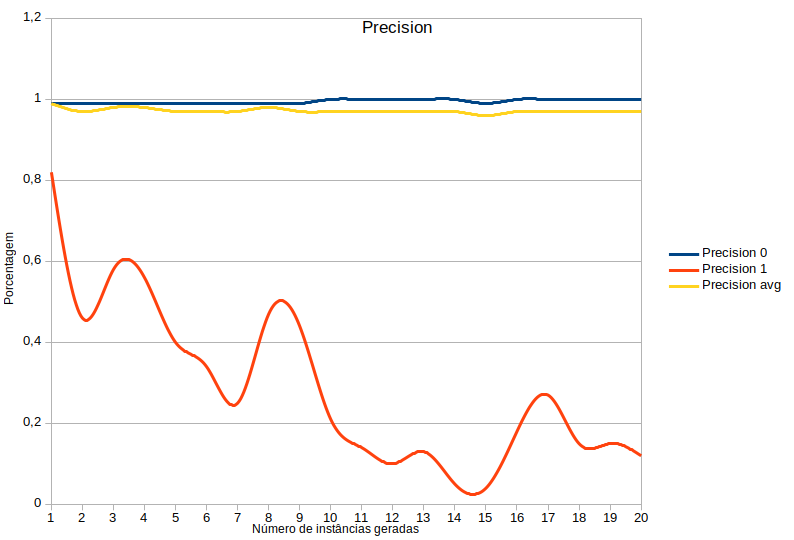
\includegraphics[scale=0.40]{./images/figura1.png} \end{center}
\end{figure}

In Figure~\ref{fig:precision}, we present the results concerning the precision. In the x-axis we have the number of instances in thousands, the y-axis represents the precision score for each class (class 0, that represents the background and class 1, that represents the plasmodium samples) and the average precision. Notice that the average precision and the class 1 precision are quite steady and quite high as we claimed. Although, as we can see the precision is decreasing for the class 1, we believe that this is due to the overfitting generated by the larger number of samples in the class 0. 

\begin{figure}[h]
\caption{Report on the recall}
\label{fig:recall}
\begin{center}
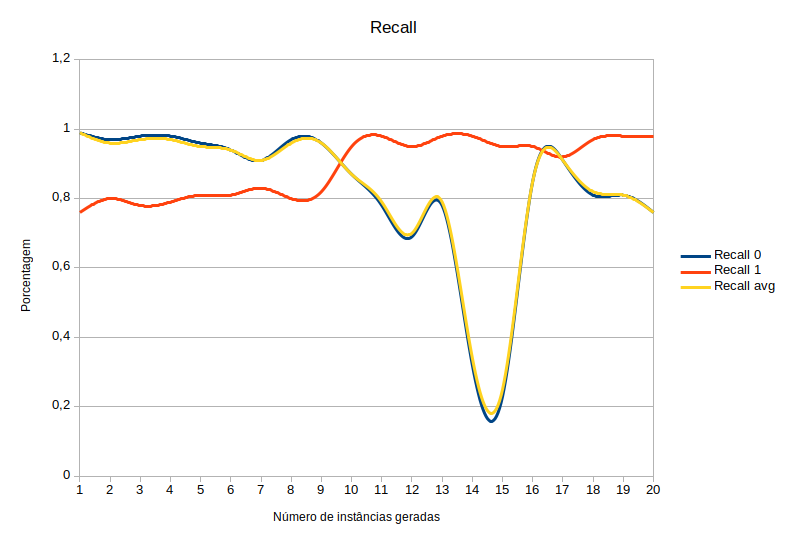
\includegraphics[scale=0.40]{./images/figura2.png} \end{center}
\end{figure}

In Figure~\ref{fig:recall}, the results concerning the recall are shown. In the x-axis we have the number of instances in thousands, the y-axis depicts the recall score for each class (class 0, representing the background and class 1, representing the plasmodium samples) and the average recall. Observe that the average recall is also quite steady and that the recall suffers the same problem of the precision due to overfitting.

\begin{figure}[h]
\caption{Report on the f1-score}
\label{fig:f1score}
\begin{center}
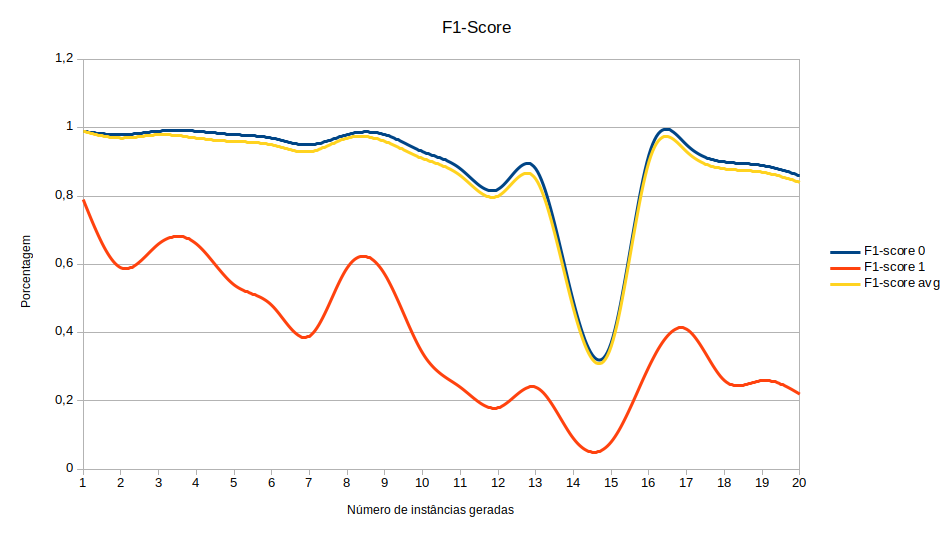
\includegraphics[scale=0.40]{./images/figura3.png} \end{center}
\end{figure}

 Finally, we present in Figure~\ref{fig:f1score} the results related to the f1-score. Again, in the x-axis we show the number of instances in thousands, the y-axis contains the f1-score score for each class (class 0, that represents the background and class 1, that represents the plasmodium samples) and the average f1-score. 




We reinforce that, as we claimed, the use of the generated samples alone are responsible for a good accuracy in the proposed CNN network model, and this process corresponds to only part of the problem of automated malaria diagnosis. There is a second challenge of choosing the best regions to be classified in the blood smear obtained. Future approaches, such as the use of YOLO or Region Based CNN, may present better results. Nevertheless, the recall and specially the f1-score tend to increase with the number of generated samples. Such behavior shows us that a fine tune is need to be able to use the generated images without loosing performance. 
\section{Conclusion}

Malaria is still a serious health problem in many areas of the world and its diagnosis is a key aspect to combat the disease. Microscopic analysis of blood samples is still the preferred method. An expert must examine several blood smears looking for parasites to declare a patient infected or not. 
This study mainly analyzes the use of DCGAN networks in object detection of malaria blood smears. Eight experiment were performed and showed that the images generated by the DCGAN network can be used in the training of a CNN network to detect objects improving classifier accuracy. We used 2200 images generated by DCGAN for training a CNN network which was tested with 600 real images, obtaining 100\% of accuracy.  
For future work, we believe that investigating more sophisticated techniques for detecting objects, such as YOLO and Region Based CNN, will be beneficial. The objects detected by the presented process can be classified allowing a new malaria diagnosis approach.

\input{sections/bib.tex}



\end{document}


